\setcounter{chaptercntr}{3}

\sectionbreak {
\gostTitleFont
\redline
\thechaptercntr . 
АНАЛИЗ И ОБРАБОТКА ДАННЫХ ПАСТЕРИЗАЦИОННОЙ УСТАНОВ-

\redline КИ
}

\titlespace

\subsection*{ 
  \gostTitleFont
  \redline
  \thechaptercntr .\thesubchaptercntr \spc
  Анализ и визуализация исходных данных технологического процесса
} \addtocounter{subchaptercntr}{1}

\subtitlespace

{\gostFont

  \par \redline Данные, которые мы будет использовать для обучения, имеют форму временных рядов, состоящих из трёх параметров. Первый параметр {--} это идентификатор датчика или исполняющего устройства, который в дальнейшем мы будем называть просто сид. Второй параметр {--} это дискретный момент времени, измеряемый в секундах. И, наконец, третий параметр {--} значение датчика. 

  \par \redline Имеющиеся данные, описывающие технологический процесс пастеризационной установки, содержат информацию от шести различных датчиков, каждый из которых описан в таблице \thechaptercntr .\thetablecntr \spc и изображён на рисунке \thechaptercntr .\theimagecntr .

	\topTablespace
	{\begin{Center}
		\par Таблица \thechaptercntr .\thetablecntr \spc {--} Описание данных ТП ПУ.

	\begin{tabular}{|c|c|c|c|}
		\hline
	  сид & Код устройства & Описание & Единица измерения \\ \hline
		1 & N101 & мощность циркуляционного насоса & \% \\ \hline
		2 & FE101 & расход молока & м$^3$/час \\ \hline
		3 & TE100 & температура гомогенизации & $^\circ$C \\ \hline
		4 & VC100 & степень открытия парового клапана & \% \\ \hline
		5 & TE101 & температура пастеризации & $^\circ$C \\ \hline
		6 & VC101 & степень открытия парового клапана & \% \\ \hline
	\end{tabular} \end{Center}} 
	\botTablespace

  \begin{sidewaysfigure}
    \centering
    \def\svgwidth{\textwidth}
    \includesvg[scale=0.6]{images/PUS.svg}
    \caption*{\gostFont Рисунок \thechaptercntr .\theimagecntr \spc {--} Схема пастеризационной установки с указанием датчиков из таблицы \thechaptercntr .\thetablecntr }
    \label{fig:NNBlackBox}
  \end{sidewaysfigure} \addtocounter{imagecntr}{1} \addtocounter{tablecntr}{1}

  \par \redline Давайте взглянем на данные с точки зрения инженерии машинного обучения и определим некоторые характеристики данных. 

  \par \redline Для начала определим, достаточно ли данных для обучения. Имеется 7 файлов формата .csv, которые хранят информацию о технологическом процессе пастеризационной установки в течении 70995465 секунд или около 835.5 дней. За такой промежуток времени мы имеем 20123304 строк данных различных сидов. Поэтому можно с уверенностью сказать, что данных для проекта машинного обучения более чем достаточно, а потому они способны обеспечить достаточную обобщающую способность при обучении модели НС.

  \par \redline Данные описывают состояние ПУ круглые сутки в течении почти двух с половиной лет. Это нам позволяет говорить о большом покрытии данных. Это значит, что данные отражают все состояния объекта. Также мы можем говорить об информативности данных, поскольку они отражают реальный технологический процесс.

  \par \redline Для прояснения дальнейших моментов, хочется в очередной раз обратить внимание на то, что данные были собраны с помощью датчиков, поэтому данные являются надёжными и не подверженными к большинству видов смещений – несогласованность данных с явлением, которые эти данные описывают.  Однако, эти данные всё-таки могут быть подвержены систематическому смещению, возникающее при измерениях или наблюдениях с помощью некоторого устройства, поскольку качество и характеристики устройства влияют на качество самих данных. Однако, мы можем игнорировать данное смещение, поскольку дальнейшая работа будет построена с теми же датчиками, а потому мы может говорить и о ещё одной черте качественных данных, а именно о том, что данные отражают реальный входы. Это значит, что будущая модель НС будет обучаться на данных, представленных в таком виде, в котором они будут в последствии приходить на входы сети. В будущем мы ещё упомянем это свойство и расскажем о некоторых подводных камнях, связанные с этим.

  \par \redline Также хочется отметить, что данные не являются результатом обратной связи, т.е. не являются результатом самой модели, поскольку при сборе данных модели ещё не существовало.

  \par \redline Для дальнейшего описания данных необходимо их визуализировать. 

  \begin{sidewaysfigure}
    \centering
    \def\svgwidth{\textwidth}
    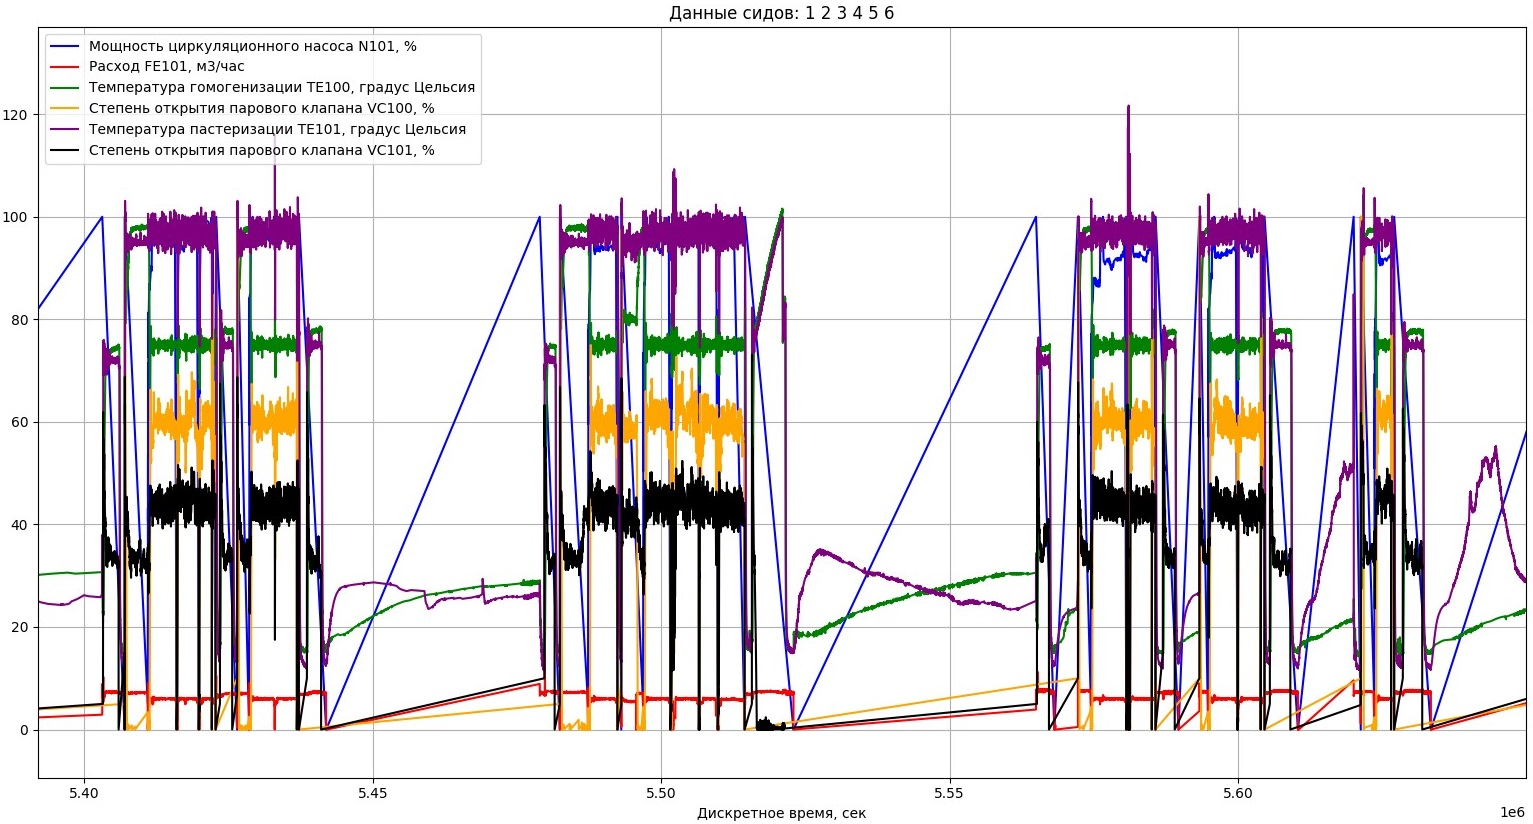
\includegraphics[scale=0.6]{images/data_1_visual.jpg}
    \caption*{\gostFont Рисунок \thechaptercntr .\theimagecntr \spc {--} Визуализация данных 1-ого файла.}
    \label{fig:Data1Visual}
  \end{sidewaysfigure} \addtocounter{imagecntr}{1}

  \begin{sidewaysfigure}
    \centering
    \def\svgwidth{\textwidth}
    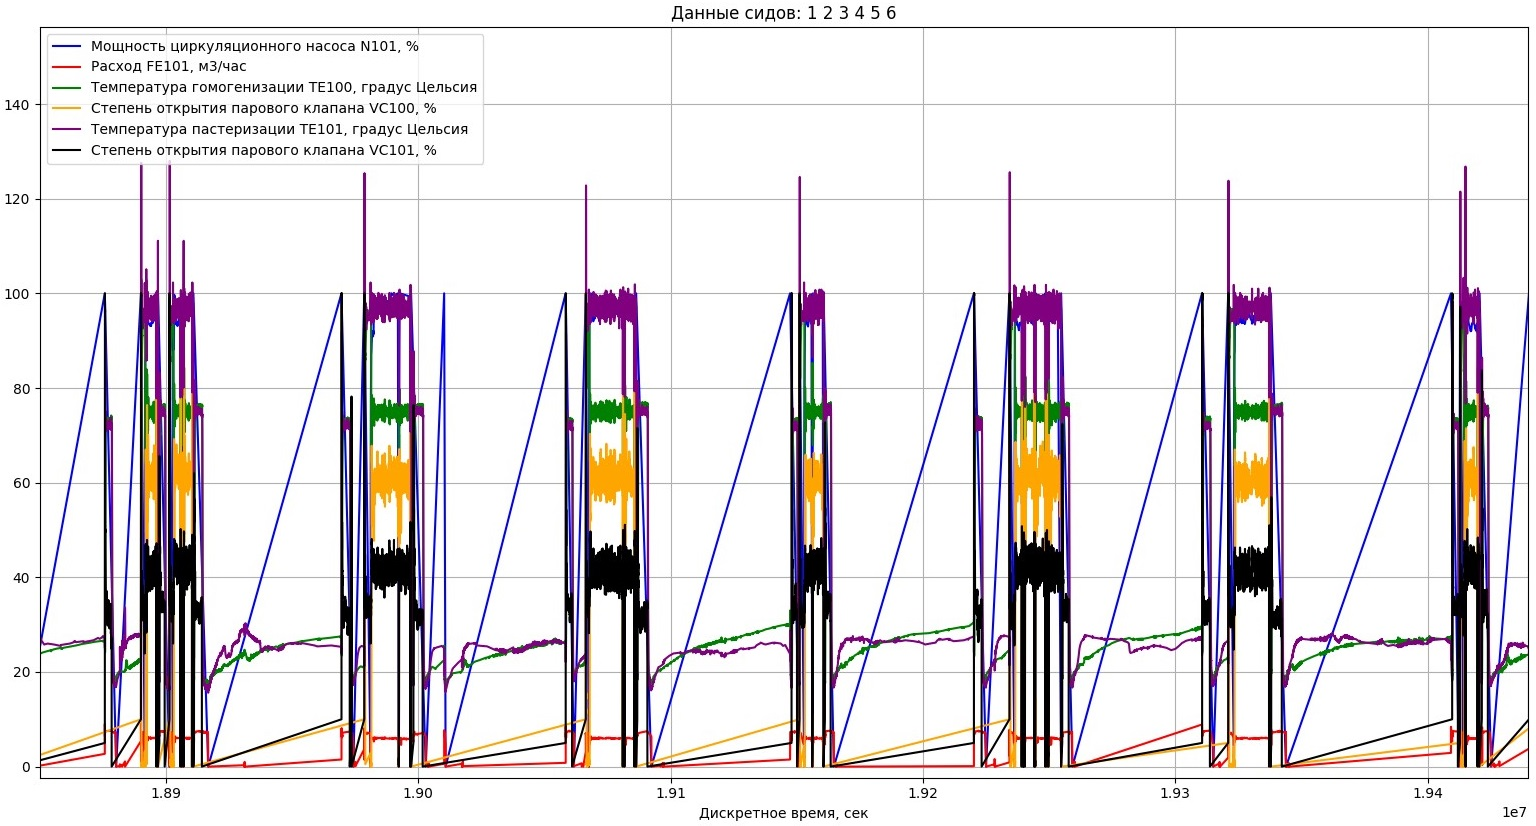
\includegraphics[scale=0.6]{images/data_2_visual.jpg}
    \caption*{\gostFont Рисунок \thechaptercntr .\theimagecntr \spc {--} Визуализация данных 2-ого файла с растянутым масштабом по оси абсцисс.}
    \label{fig:Data2Visual}
  \end{sidewaysfigure} \addtocounter{imagecntr}{1}

  \begin{sidewaysfigure}
    \centering
    \def\svgwidth{\textwidth}
    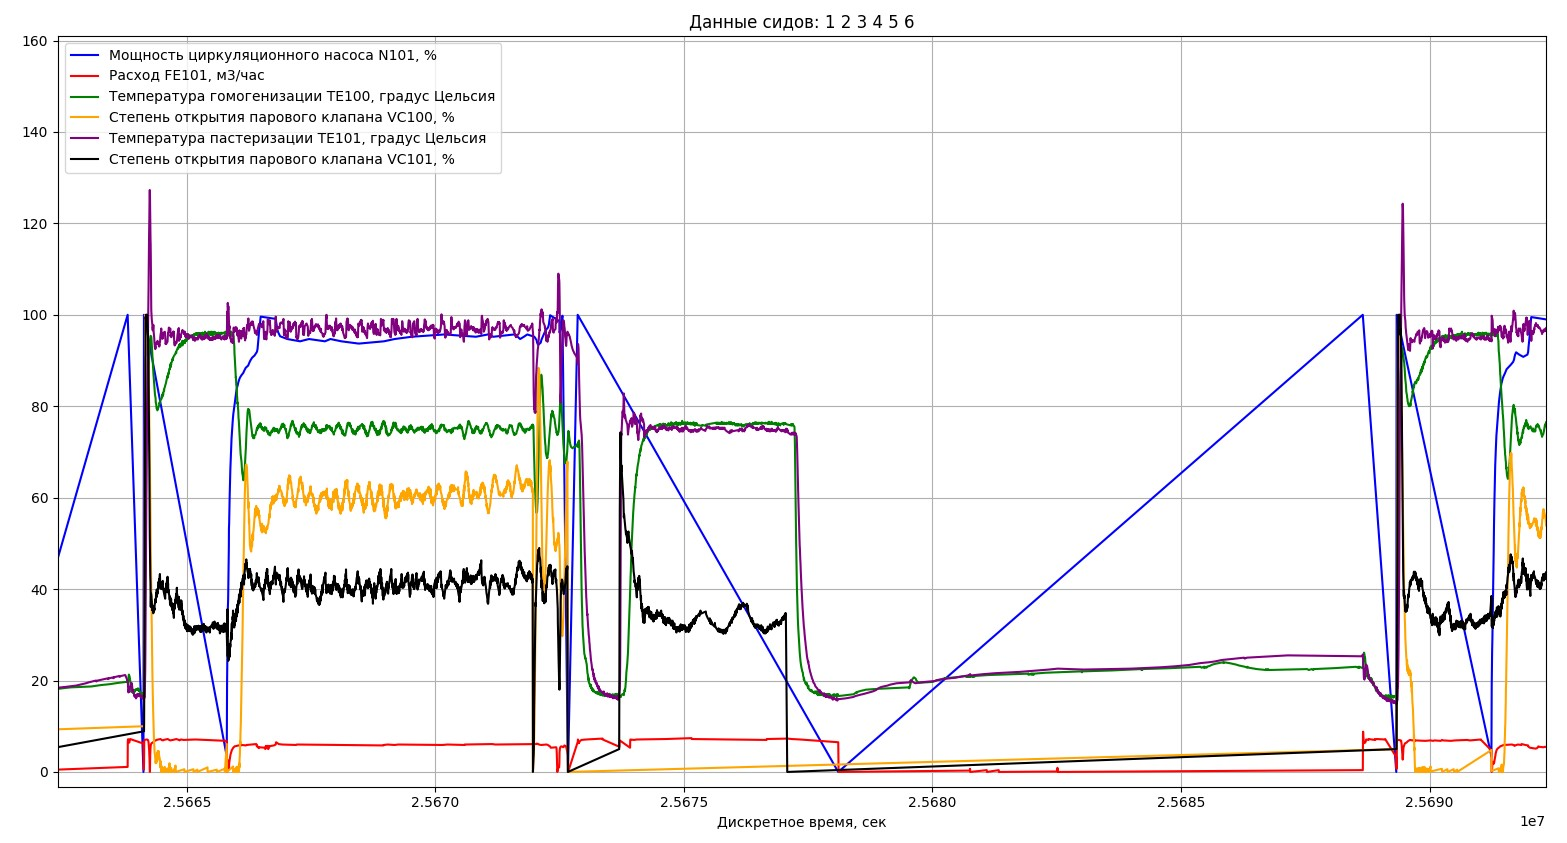
\includegraphics[scale=0.6]{images/data_3_visual.jpg}
    \caption*{\gostFont Рисунок \thechaptercntr .\theimagecntr \spc {--} Визуализация данных 3-ого файла с cуженным масштабом по оси абсцисс.}
    \label{fig:Data3Visual}
  \end{sidewaysfigure} \addtocounter{imagecntr}{1}

  \begin{sidewaysfigure}
    \centering
    \def\svgwidth{\textwidth}
    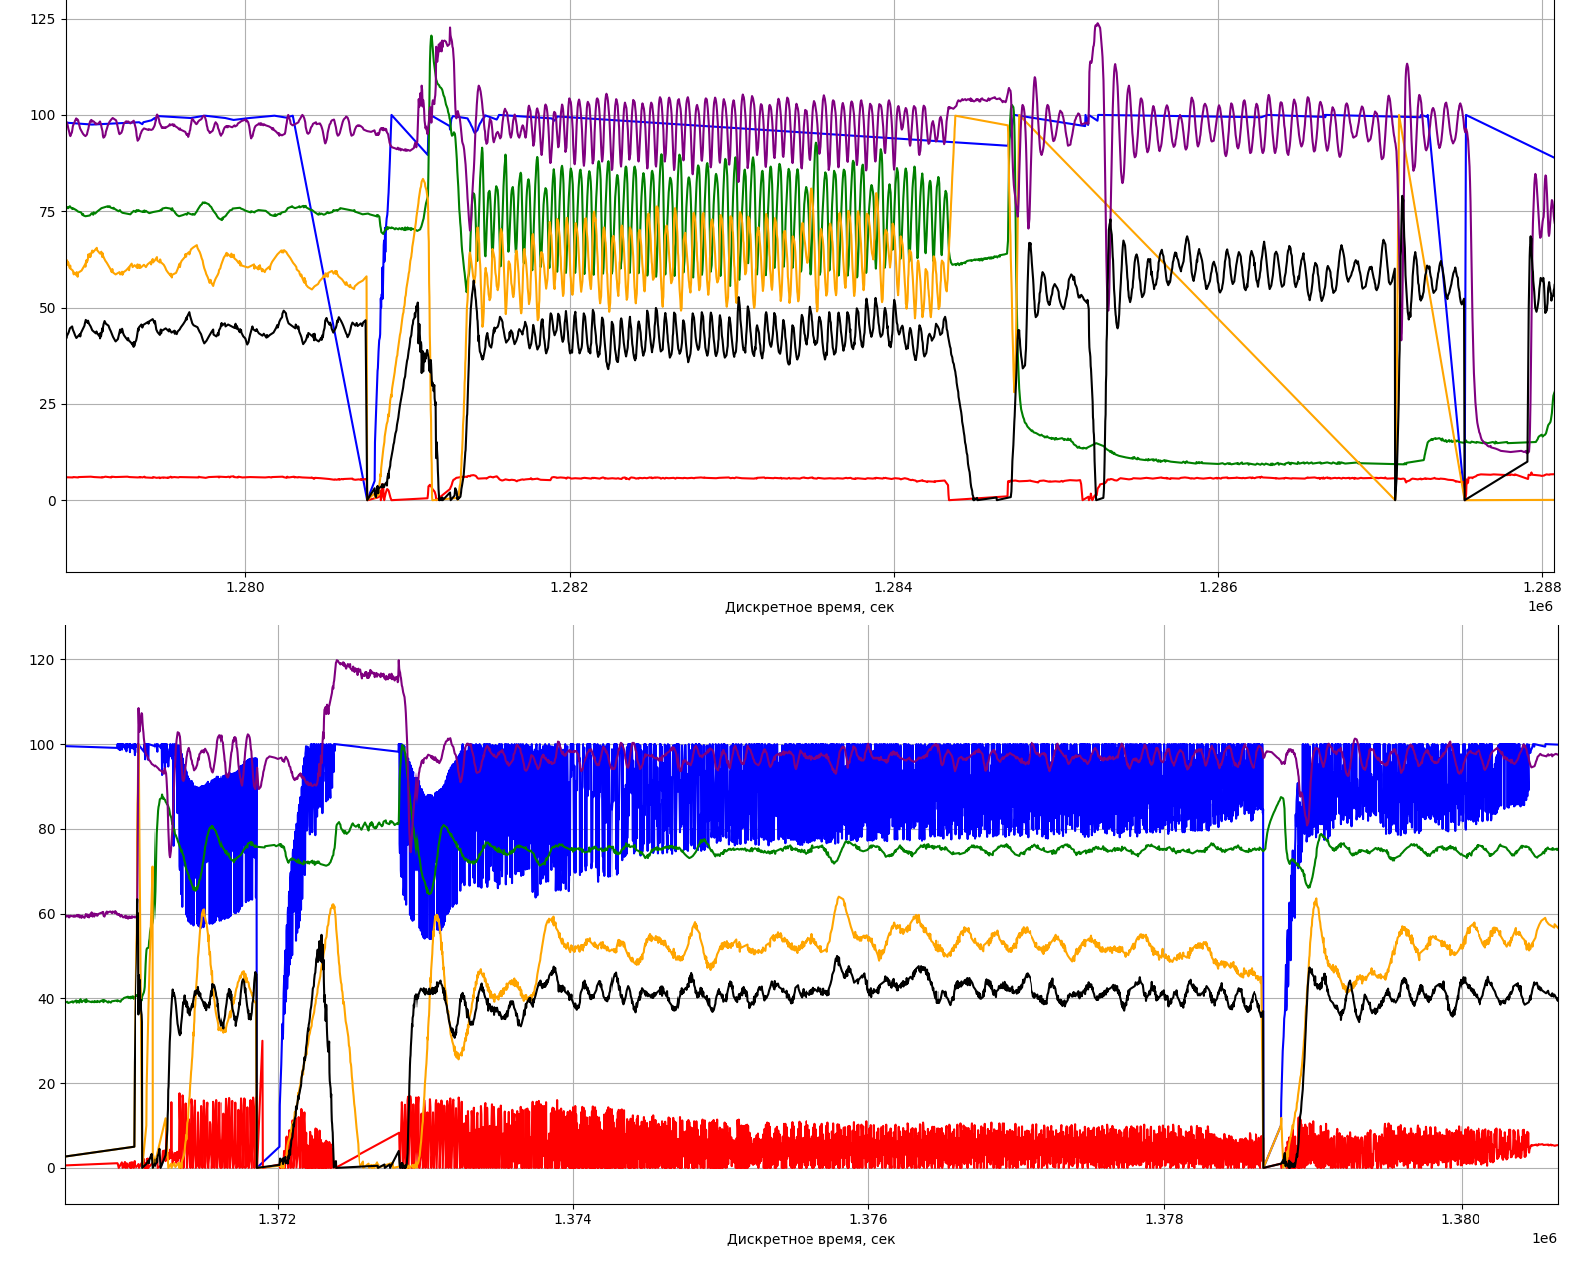
\includegraphics[scale=0.5]{images/data_1_anomaly.png}
    \caption*{\gostFont Рисунок \thechaptercntr .\theimagecntr \spc {--} Визуализация данных 1-ого файла с примерами нестандартного поведения системы.}
    \label{fig:Data1VisualAnomaly}
  \end{sidewaysfigure} \addtocounter{imagecntr}{1}

  \par \redline Сравнивая данные на рисунках 3.2, 3.3 и 3.4, хотелось бы пояснить, что данные остальных файлов очень схожи с данными на представленных рисунках. Однако, как можно увидеть на рисунке 3.5, данные могут содержать непохожее на другие участки поведение. Такое будет называться аномалией. При этом такие аномалии встречаются только в первом .scv файле, поскольку схожее поведение пастеризационной установки средствами визуализации в других файлах выявлено не было. Это значит, что мы имеем большинство данных без аномалий, но также имеем и примеры данных с аномалиями. 

  \par \redline Поэтому первый .csv файл для обучения рассматриваться не будет, поскольку необходимо прогнозировать правильное поведение системы, которое не содержит отклонений. 

  \par \redline Теперь пришло время определить связи между параметрами пастеризационной установки. Беря во внимание всю собранную о данных и самой пастеризационной установки информацию, а также общение с персоналом, ответственные за работу установки, удалось более подробно сформулировать задачу данной работы. Необходимо прогнозировать технологический процесс пастеризационной установки, но это подразумевает прогнозирование трёх величин: расход, температура гомогенизации и температура пастеризации. В случае же с параметрами, описывающими степень открытия паровых клапанов и мощность циркуляционного насоса, то их прогнозировать нет необходимости, поскольку они изменяются в зависимости от сигналов регуляторов. 

  \par \redline Таким образом, параметр мощности напрямую влияет на параметр расхода. Чем больше мощность насоса, тем больше расход молока. Однако, может быть такой момент, когда насос работает на полную мощность, а расход падает или равен нулю. Ответом на эту ситуацию служит тот факт, что в танке, из которого насос подкачивает молоко, собственно говоря, молока нет. Однако данной информацией о том, если ли молоко в танке, исходные данные не располагают. В таком случае, если мощность насоса не будет влиять на расход молока, то результаты прогноза и реальные данные будут значительно расходиться и это должно будет быть определено как аномалия. 
  
  \par \redline Параметр температуры гомогенизации напрямую зависит от степени открытия парового клапана. Пар нагревает молоко, отдавая ему свою температуру, поэтому пар должен непрерывно циркулировать в системе при нагревании молока. В этом нам помогает паровой клапан, который способен препятствовать потоку пара, либо наоборот, дать ему возможность циркулировать в системе. Такая же история и с температурой пастеризации. Тоже существует секция с паром, влияющая на температуру молока при пастеризации. 
  
  \par \redline Также можно создать дополнительные связи: параметр температуры гомогенизации зависит от параметра расхода и параметр температуры пастеризации зависит от температуры гомогенизации. Но параметр расход и параметр температуры гомогенизации также влияет и на степени открытия паровых клапанов, поэтому данные связи будут опущены, поскольку они учтены в других сидах, имеющих более тесные связи с прогнозируемыми величинами.    

  \par 
}

\titlespace

\subsection*{ 
  \gostTitleFont
  \redline
  \thechaptercntr .\thesubchaptercntr \spc
  Обработка данных и их подготовка к прогнозированию
} \addtocounter{subchaptercntr}{1}

\titlespace

{\gostFont

  \par \redline И так, пришло время поговорить об обработке данных. Она нужна в основном для того, чтобы сделать данные понятными для модели, а также для заполнения «дыр» в данных или для различного рода аппроксимаций. Под «дырами» понимаются некоторые пропущенные значения, например, определено время и значение датчика, а сид пропущен, вместо него пустое поле. Также под «дырами» понимаются магические числа, вроде -1, 99999 и другие, говорящие о том, что значение, заменённое магическим числом, неизвестно, но пустого поля быть не может. В данных строчного формата, а это в таком, в котором хранятся исходные данные, такой проблемы не наблюдается, однако не стоит об этом забывать. В будущем с этим придётся столкнуться.

  \par \redline Поговорим о хранении данных. Начальные данные хранятся в файлах формата .csv. Это весьма распространённый формат файлов для хранения данных, представленных в форме временных рядов. В них данные хранятся в следующем виде: 

  \formulaspace
  \begin{Center}
  <сид>;<время>;<значение>. 
  \end{Center}
  \formulaspace

  \par \redline В дальнейшем такой вид данных мы будем обозначать как ocdf-формат данных. Преимуществом хранения данных в таких файлах является их доступность для любых программ или языков. Однако такие файлы занимают большой объём, а также при работе с такими файлами чтение или запись информации занимает большое количество времени.  

  \par \redline Для решения основных проблем при работе с файлами формата .csv, было принято решение использовать бинарные файлы формата .bin для хранения данных. Это дало возможность уменьшить занимаемый объём файлов, но самое главное, это позволило значительно сократить время для записи или чтения информации. 

  \par \redline В ходе работы с моделью возможно не будет необходимости работать со всеми сидами, а только с определёнными. Для того, чтобы не задействовать оперативную память зря, необходимо разделить данные по сидам. Поэтому были реализованы функции парсинга данных.

  \par \redline Для формирования различных наборов данных необходима возможность обрезать данные до необходимого нам диапазона, количества или момента времени. Для более полного понимая смысла обрезки данных в очередной раз обратимся к инженерии машинного обучения: весь набор данных делится на обучающий, контрольный и тестовый наборы. Обучающий набор используется для непосредственного обучения модели. На контрольном наборе проверяется качество модели и подбираются её параметры, другими словами, настраивается модель. На тестовом наборе проверяется работа сети и делается вердикт о готовности модели. 

  \par \redline Для формирования различных наборов данных как раз и нужны различные способы обрезки данных, позволяющие отбросить данные как справа, так и слева. 
 
  \par \redline Также необходима возможность добавлять новые данные, чтобы при обучении сеть, которая учитывает зависимости между различными датчиками, была обеспечена данными необходимых сидов.  

  \par \redline Учитывая особенности вида данных, которые поступают на предиктовый детектор системы Kaspersky MLAD, а также ввиду того, что данная модель будет работать в режиме реального времени и данные будут поступать через некоторый промежуток времени, то необходимо сделать так, чтобы начальные данные также были равноудалены друг от друга относительно оси времени. Однако, взаимное удаление точек по оси времени в начальных данных не постоянно. Эти диапазоны необходимо выровнять, чтобы повысить схожесть реальных входов и входов при обучении модели. Другими словами, необходимо преобразовать начальный данные в такие данные, в которых каждое значение времени представляло собой арифметическую прогрессию. Вышесказанное описывает формула (\thechaptercntr .\theformulacntr):

	\formulaspace \par \redline 
    $t_i = t_0 + i \cdot r$
	  \hfill (\thechaptercntr .\theformulacntr) \redline
	\formulaspace \addtocounter{formulacntr}{1}

  \begin{tabular}{p{0,875cm}p{0,3cm}p{15,175cm}}
		& где  & $t_0$ {--} начальное значение времени; \\
		& 	   & $r$ {--} необходимое расстояние между точками, представляющее собой некоторую константу, которую может задать пользователь; \\
    & 	   & $i$ {--} номер точки, итерации, элемента прогрессии; $t_i$ {--} i-ыт элемент прогрессии.  \\
    & 	   & $t_i$ {--} i-ыт элемент прогрессии. \\
  \end{tabular}

  \par \redline Теперь осталось определить значение ординаты для каждого рассчитанного значения времени. Для этого было принято решение воспользоваться аналитической геометрией и взять за основу уравнение прямой, проходящей через две точки. Это уравнение представлено в формуле (\thechaptercntr .\theformulacntr):  

  \formulaspace \par \redline 
    $\scaleto{\frac{x - x_1}{x_2 - x_1} = \frac{y - y_1}{y_2 - y_1}}{22pt}$
    \hfill (\thechaptercntr .\theformulacntr) \redline
  \formulaspace \addtocounter{formulacntr}{1}

  \begin{tabular}{p{0,875cm}p{0,3cm}p{15,175cm}}
		& где  & точка $\left(x, y\right)$ {--} это точка, которую необходимо найти между точками $\left(x_1, y_1\right)$ и $\left(x_2, y_2\right)$, взятых из реальных данных. \\
  \end{tabular}

  \par \redline Про соотношение этих точек известно, что $x_1 \leq x \leq x_2$. 

  \par \redline Для определение ординаты для i-того элемента прогрессии необходимо взять две ближайших точки из реальных данных относительно оси абсцисс к искомой точке. Тогда для определения ординаты имеем формулу (\thechaptercntr .\theformulacntr):

  \formulaspace \par \redline 
    $y = \left(\scaleto{\frac{\left(x - x_1\right) \cdot \left(y_2 - y_1\right)}{x_2 - x_1}}{24pt}\right) + y_1$
    \hfill (\thechaptercntr .\theformulacntr) \redline
  \formulaspace \addtocounter{formulacntr}{1}

  \par \redline Таким образом можно получить аппроксимированные данные, где взаимное удаление между двумя соседними точками будет везде постоянным.  

  \par \redline Благодаря возможности выравнивания диапазонов по оси абсцисс, появляется возможность создать, так называемые, аккуратные данные – данные представленные в виде упорядоченной таблицы без каких-либо «дыр». Однако, если попытаться перевести имеющиеся данные в табличный формат, который в последствии мы будем называть tdf-форматом, то мы обнаружим, что начальные данные содержат информацию о значениях датчика при неповторяющихся уникальных значениях времени. Это значит, что если для некоторого датчика определено его значение в некоторый момент времени в начальных данных, то значение других датчиков в этот же момент времени не известно. Для решения данной проблемы нам помогут операции парсинга и выравнивания диапазонов по оси абсцисс. Чтобы преобразовать данные формата ocdf в данные формата tdf необходимо выполнить несколько последовательных действий. 

  \par \redline Для начала необходимо убедиться, что данные формата ocdf содержат в себе данные всех сидов, а после распарсить данные по сидам. Затем обрезать все последовательности распарсенных данных с их начала и до максимального значения времени первых элементов последовательности распарсенных данных, также с минимального значения времени последних элементов последователи распарсенных данных до конца всех последовательностей распарсенных данных. Если в обрезаемой последовательности нет точки с граничным значением времени, тогда необходимо найти эту точку средствами уравнения прямой через две точки, описанной выше. Далее выровнять диапазоны по оси абсцисс для всех расперсенных данных. В заключении требуется соединить полученные данные в одну последовательность следующего вида. Таким образом, строка данных формата tdf будет состоять из параметра времени и параметров всех шести датчиков, значение которых определено в данный момент времени. 

  \par \redline Выполнив алгоритм, мы получаем аккуратные данные в табличном виде. Хранить их предпочтительно в бинарном виде, поскольку в формате .csv такие данные будут занимать очень много места, да и время на их чтение или запись будет довольно-таки немаленьким. 

  \par \redline Учитывая некоторые особенности активирующих функций, некоторые модели будут содержать в себе встроенные модули преобразования данных из одного диапазона по оси ординат в эквивалентные данные из другого диапазона по оси ординат и наоборот, сохраняя значения по оси абсцисс. Такая операция привидения данных к определённому диапазону значений в дальнейшем будет называеться скейлингом.

  \par \redline Данная задача выглядит следующим образом: пусть есть $y \in \left[a; b\right]$, а необходимо преобразовать $y$ в эквивалентное значение $z \in \left[c; d\right]$. Тогда для операции скейлинга имеем формулу (\thechaptercntr .\theformulacntr):

  \formulaspace \par \redline 
    $z = \scaleto{\frac{\left(y - a\right) \cdot \left(b - a\right)}{d - c}}{22pt} + c$
    \hfill (\thechaptercntr .\theformulacntr) \redline
  \formulaspace \addtocounter{formulacntr}{1}

  \par \redline А для того, чтобы восстановить эти значения, т.е. провести операцию обратного скейлинга, необходимо использовать формулу (\thechaptercntr .\theformulacntr): 

  \formulaspace \par \redline 
    $y = \scaleto{\frac{\left(z - c\right) \cdot \left(d - c\right)}{b - a}}{22pt} + a$
    \hfill (\thechaptercntr .\theformulacntr) \redline
  \formulaspace \addtocounter{formulacntr}{1}

  \par \redline Операции скейлинга предполагают те модели, выходные элементы которых используют активирующие функции, имеющие горизонтальные асимптоты. Другими словами, активирующие функции, ограниченные по оси ординат. В таком случае, перед обучение или прогнозированием данных, будет проведена операция скейлинга, после основная операция, а в завершении операция обратного скейлинга. Т.к. данные уже изучены, можно с полной уверенность сказать, что операцию скейлинга для данных по оси ординат мы можем провести. 

  \par
}

\setcounter{subchaptercntr}{1}
\setcounter{formulacntr}{1}
\setcounter{imagecntr}{1}
\setcounter{tablecntr}{1}
